\documentclass[sigconf,nonacm]{acmart}
\settopmatter{printacmref=false}
\renewcommand\footnotetextcopyrightpermission[1]{}
\pagestyle{plain}

\usepackage{booktabs}
\usepackage{graphicx}
\usepackage{amsmath}

\newcommand{\cpuname}{Intel(R) Xeon(R) Processor @ 2.10GHz}
\newcommand{\osname}{Linux-6.18.44-fc-v42-x86\_64-with-glibc2.39}
\newcommand{\pyver}{3.12.3}
\newcommand{\npver}{2.4.4}
\newcommand{\spver}{1.17.1}
\newcommand{\repeats}{15}


\begin{document}

\title{Efficiency and Robustness of Pad\'e-Accelerated Newton Methods for Nonlinear Systems}
\subtitle{An Extension of the $(p,q)$-Parametrized Iterative Family of Herceg et al.\ (2025)}

\author{Roni Datta (2105148)}
\affiliation{\institution{Department of CSE}\city{Dhaka}\country{Bangladesh}}
\author{Shaikh Fardin Hasib (2105146)}
\affiliation{\institution{Department of CSE}\city{Dhaka}\country{Bangladesh}}
\author{Sarowar Alam Roki (2105129)}
\affiliation{\institution{Department of CSE}\city{Dhaka}\country{Bangladesh}}
\author{Sajid Hasan (2105145)}
\affiliation{\institution{Department of CSE}\city{Dhaka}\country{Bangladesh}}
\author{S.M Muttakin Islam (2105136)}
\affiliation{\institution{Department of CSE}\city{Dhaka}\country{Bangladesh}}

\renewcommand{\shortauthors}{Datta et al.}

\newcommand{\groupno}{10}

\begin{abstract}
Herceg et al.\ (\textit{Mathematics}, 2025) build a family of iterative methods for systems of
nonlinear equations by replacing the square root in Cauchy's method with a Pad\'e
approximant of order $(p,q)$, giving convergence order $\min\{p+q+2,4\}$. The paper proves
this order and demonstrates it with fixed-size examples in high-precision arithmetic, but does
not measure double-precision wall-clock cost against problem size, and assumes throughout
that the Jacobian is nonsingular. We reimplement the family in NumPy/SciPy and test both
gaps. First, on five systems (sizes 21--1601) we time every $(p,q)$ up to $(2,1)$: the direct
implementation, which forms an $n\times n$ matrix $\Lambda$ every step, is 3--5$\times$ slower
than Newton at $n=401$ despite needing fewer iterations, because that matrix costs an extra
$O(n^3)$ solve. A second, mathematically equivalent implementation that avoids forming
$\Lambda$ is faster: for $(2,0)$ it drops below Newton's time for $n\gtrsim 600$, the only case
in our tests where a higher-order member is actually cheaper in wall-clock terms. Second, on a
parametrized near-singular system, a singular Chandrasekhar H-equation, and two classical
singular-Jacobian problems (Powell, cosine-diagonal), we compare plain LU against truncated
SVD (TSVD) and Levenberg--Marquardt (LM) solves. LU is enough for mildly ill-conditioned
problems but fails completely (0\% success) on the exactly singular H-equation, where TSVD
succeeds every time. LM is unreliable throughout: it stalls or diverges even for Newton itself
once the Jacobian is within about $10^{-8}$ of singular. We report the numbers directly,
including the cases where the paper's own results did not exactly reproduce in double
precision.
\end{abstract}

\maketitle
\begin{center}\small
CSE402: Numerical Analysis, Simulation and Modeling Sessional \\
Section C1 \quad Group \groupno{} \quad Department of CSE
\end{center}

\section{Introduction and Base Paper Review}

Newton's method for $F(x)=0$, $F:\mathbb{R}^n\to\mathbb{R}^n$, converges quadratically near a
simple root. Cauchy's method reaches cubic order by adding a square-root correction, but the
square root and a second-derivative term make it expensive. Herceg, Herceg, Odry and
Tadi\'c~\cite{herceg2025pade} replace the square root with a Pad\'e rational approximant
$\varphi_{p,q}$ of $2/(1+\sqrt{1-2z})$ and a curvature surrogate
$\Lambda(x)=\tfrac32\big(I-F'(x)^{-1}F'(y)\big)$, $y=x-\tfrac23F'(x)^{-1}F(x)$, giving the step
\[
x_{k+1}=x_k-\Phi_{p,q}\big(\Lambda(x_k)\big)\,F'(x_k)^{-1}F(x_k),
\]
where $\Phi_{p,q}(\Lambda)=B_{p,q}(\Lambda)^{-1}A_{p,q}(\Lambda)$ and $A_{p,q}$, $B_{p,q}$ are
the numerator and denominator polynomials of $\varphi_{p,q}$ evaluated at the matrix
$\Lambda$. $(p,q)=(0,0)$ is Newton's method; $(1,1)$ is Jarratt's classical fourth-order
method~\cite{jarratt1966}. The paper proves order $\min\{p+q+2,4\}$ under the standard
assumption that $F'$ is continuous and nonsingular at the root, and confirms it with
20{,}000-digit Mathematica arithmetic on fixed-size test systems, several with over a hundred
unknowns.

The paper does not address two questions that matter for anyone who would actually use these
methods: whether the higher iteration order still pays off once it is measured in wall-clock
time rather than iteration count, since $\Lambda$ costs a full matrix solve to build; and how
the family behaves once the nonsingularity assumption is violated or nearly violated, which is
exactly where a cheap, robust solver matters most. Both questions are ordinary engineering
questions about a mathematically sound method, and both have clear, checkable answers, so we
treat them as the two goals of this project: (1) benchmark the order/cost trade-off in double
precision as $n$ grows, and (2) test the family under increasing Jacobian ill-conditioning with
three linear-solve strategies (LU, truncated SVD, Levenberg--Marquardt).

\section{Methodology}

\paragraph{Two implementations of one iteration.}
Reading the paper literally, every step needs $\Lambda(x)=\tfrac32(I-F'(x)^{-1}F'(y))$, an
$n\times n$ matrix, which costs one $O(n^3)$ solve with $n$ right-hand sides beyond the Newton
direction itself. We call this the \emph{generic} form; it is what any direct translation of
the formulas in the paper would produce, and it is required whenever $q\ge2$, since $B_{p,q}$
is then a genuine matrix polynomial in $\Lambda$. For $q=0$, however, $\Phi_{p,0}(\Lambda)$ is
just a polynomial in $\Lambda$ applied to a vector, so it can be computed as $p$ repeated
vector solves $\Lambda t=\tfrac32\big(t-F'(x)^{-1}(F'(y)\,t)\big)$ without ever forming
$\Lambda$ as a matrix; we call this the \emph{cheap} form. For $(1,1)$ the family reduces
algebraically to $(6F'(y)-2F'(x))^{-1}(3F'(y)+F'(x))\,F'(x)^{-1}F(x)$, Jarratt's original
two-solve formula~\cite{jarratt1966}, which is also cheap. \texttt{tests/test\_core.py} checks
that the cheap and generic forms give identical iterates. Both use LU factorization with
partial pivoting for every linear solve, as the paper specifies.

\paragraph{Cost model.} We count leading-order multiplications and divisions per iteration.
Newton is $\tfrac13n^3+n^2$ (one LU, one solve). The generic $(p,q)$ member with $q\ge1$ needs
two Jacobian factorizations, one $n$-right-hand-side solve to build $\Lambda$ ($n^3$), up to
$p$ matrix-vector products, and, for $q\ge2$, up to $q-1$ matrix-matrix products ($n^3$ each)
plus a second factorization for $B_{p,q}(\Lambda)$. The cheap forms drop the $n^3$ solve for
$\Lambda$ entirely.

\paragraph{Solvers under ill-conditioning.} \texttt{padenewton/linsolve.py} implements
LU (baseline, no protection against near-singularity), TSVD (Moore--Penrose pseudo-inverse with
singular values below a relative threshold discarded), and LM
(solve $(J^\top J+\lambda I)\Delta=J^\top f(x)$ with $\lambda=\|f(x)\|_2^2$, which vanishes at
the root, following Yamashita and Fukushima~\cite{yamashita2001}). A fourth variant, LM-N, uses
the LM-damped solve only for the Newton direction $F'(x)^{-1}f(x)$ and an exact LU solve for
$F'(x)^{-1}F'(y)$ inside $\Lambda$; it isolates whether damping the curvature term specifically,
as opposed to damping generally, is what causes trouble for $q\ge1$ members.

\section{Implementation and Experiments}

All code is Python 3.12 with NumPy~\cite{numpy} \pyver, SciPy~\cite{scipy} \spver, and mpmath for
the high-precision checks. Pad\'e coefficients are computed once in exact rational arithmetic
(\texttt{fractions.Fraction}) and cross-checked against Table 2 of the paper. Timings use a
single BLAS thread and report the median of \repeats{} repeated, interleaved runs per
$(\text{system},n,p,q)$ combination (5 repeats at $n\ge601$), on \cpuname. Six unit tests cover
the Pad\'e coefficients, the order-$(p{+}q{+}1)$ agreement of $\varphi_{p,q}$ with the exact
function, convergence on a base-paper system, agreement of the cheap and generic forms, and
agreement of the four solvers on a well-conditioned problem.

\paragraph{Validation.} We reproduce Table 5 of the paper (Example 1, cases 1a--1g) with the
literal stopping rule $\|F(x^{(k)})\|_\infty+\|x^{(k)}-x^{(k-1)}\|_\infty<10^{-12}$.

\paragraph{Order of convergence.} With mpmath at 1500 decimal digits we run every member up to
$(1,2)/(2,1)$ on three of the paper's Example-1 systems and compute the computational order of
convergence $\mathrm{COC}_k=\ln(e_{k+1}/e_k)/\ln(e_k/e_{k-1})$, $e_k=\|x_k-\alpha\|_\infty$,
taking $\alpha$ from 90 Newton steps at the same precision.

\paragraph{Efficiency.} Five systems: the paper's own cyclic-product system (1f) and cyclic-cubic
system (7c), the Bratu boundary-value problem~\cite{bratu1914}, the Chandrasekhar
H-equation~\cite{chandrasekhar1960} at $c=0.99$, and the More--Garbow--Hillstrom trigonometric
system~\cite{morgarhil1981}. Sizes $n\in\{21,51,101,201,301,401\}$ for every $(p,q)$ up to
$(2,1)$, generic and cheap forms; sizes $n\in\{601,801,1201,1601\}$ for Newton and the cheap
forms only, since the generic form's $n^3$ solve for $\Lambda$ becomes too slow to run
repeatedly at that size.

\paragraph{Robustness.} A parametrized near-singular system
$f_1=x+y-2,\ f_2=(x-1)+(1+\epsilon)(y-1)+(y-1)^3$, with $\det F'(\text{root})=\epsilon$, at
$\epsilon\in\{10^{-2},10^{-4},10^{-6},10^{-8},10^{-10}\}$ and 100 random starts per $\epsilon$.
(The proposal's system was purely linear, so $F'(y)=F'(x)$ identically and $\Lambda\equiv0$,
collapsing every $(p,q)$ member to Newton; the cubic term above avoids that while keeping
$\det F'(\text{root})=\epsilon$.) We also test three systems whose Jacobian is exactly singular
at the solution: Powell's four-dimensional function~\cite{powell1970}, a 20-dimensional
cosine-diagonal system $x_i-1.5\sin(\sum_{j\ne i}x_j)=0$, and the H-equation at $c=1$ (100 random
starts each). A run counts as \emph{accurate} if the forward error to the known root is below
$10^{-6}$ (for the H-equation at $c=1$, no closed-form root is used; accurate means the residual
stopping rule was met with residual below $10^{-10}$). We additionally sweep the TSVD threshold
against $\epsilon$ to see whether TSVD's apparent robustness is intrinsic or an artifact of the
fixed threshold matching the fixed $\epsilon$ values used elsewhere.

\section{Results and Discussion}

\subsection{Validation against the base paper}

Table~\ref{tab:validation} compares our iteration counts (left of each slash) against the
paper's Table 5 (right of each slash), same stopping rule, same starting points. Twelve of
fifteen cases match exactly. Three do not: 1a-2, 1b-2 and 1c-2 all show our Newton method taking
one extra iteration. To rule out double-precision rounding as the cause, we reran plain Newton
on those three cases in 50-digit mpmath arithmetic (\texttt{padenewton/mpsystems.py}): the
iteration counts were identical to our double-precision run, not the paper's. So the discrepancy
is not a precision artifact on our end; it is most likely a difference in how the paper counted
iterations or evaluated the stopping rule for those three cases, which we cannot resolve without
their code. We report this rather than silently matching the table.

\begin{table}[t]
\caption{Iterations to converge: ours / paper's Table 5. Newton, third-order PM(3) (best
$(0,1)$/$(1,0)$), best fourth-order PM(4) found by search over $(p,q)\in\{0..4\}^2$.}
\label{tab:validation}
\small
\begin{tabular}{lccc}
\toprule
case & Newton & PM(3) & PM(4) best \\
\midrule
1a-1 & 10 / 10 & 7 / 7 & 4 / 4 \\
1a-2 & 8 / 7 & 5 / 5 & 4 / 4 \\
1a-3 & 5 / 5 & 4 / 4 & 4 / 4 \\
1b-1 & 7 / 7 & 5 / 5 & 4 / 4 \\
1b-2 & 6 / 5 & 4 / 4 & 3 / 3 \\
1c-1 & 7 / 7 & 5 / 5 & 4 / 4 \\
1c-2 & 6 / 5 & 4 / 4 & 3 / 3 \\
1d-1 & 5 / 5 & 4 / 4 & 3 / 3 \\
1d-2 & 6 / 6 & 5 / 5 & 3 / 3 \\
1e-1 & 6 / 6 & 4 / 4 & 4 / 4 \\
1e-2 & 5 / 5 & 3 / 3 & 3 / 3 \\
1f-1 & 6 / 6 & 4 / 4 & 3 / 3 \\
1f-2 & 7 / 7 & 5 / 5 & 3 / 3 \\
1g-1 & 6 / 6 & 4 / 4 & 3 / 3 \\
1g-2 & 7 / 7 & 5 / 5 & 3 / 3 \\
\bottomrule
\end{tabular}

\end{table}

\subsection{Order of convergence}

Table~\ref{tab:coc} shows the last well-resolved COC value (excluding iterations where the error
is already below the working precision floor) for each member. Every value matches the proven
order $\min\{p+q+2,4\}$ to within 0.03, except system 1g at $(1,2)$ and $(2,1)$, where we get
5.05 instead of 4. This is not a contradiction of the theorem: Theorem 1 gives $\min\{p+q+2,4\}$
as a guaranteed order, not an exact one, and superconvergence at a specific point for a specific
system is possible when the asymptotic error constant $E_{p,q}$ happens to vanish there. We did
not chase this further; it does not affect the wall-clock comparison, which is the point of this
project.

\begin{table}[t]
\caption{Computational order of convergence at 1500 decimal digits, last well-resolved
iteration, against the proven order $\min\{p+q+2,4\}$.}
\label{tab:coc}
\small
\begin{tabular}{lcccc}
\toprule
(p,q) & theory & 1a & 1b & 1g \\
\midrule
(0,0) & 2 & 2.00 & 2.00 & 2.00 \\
(0,1) & 3 & 3.00 & 3.00 & 3.01 \\
(1,0) & 3 & 3.00 & 3.00 & 3.01 \\
(1,1) & 4 & 4.00 & 4.00 & 4.02 \\
(1,2) & 4 & 4.00 & 4.00 & 5.05 \\
(2,0) & 4 & 4.00 & 4.00 & 4.02 \\
(2,1) & 4 & 4.00 & 4.00 & 5.05 \\
\bottomrule
\end{tabular}

\end{table}

\subsection{Efficiency: does the higher order pay off?}

Figure~\ref{fig:eff-rel} plots wall-clock time relative to Newton at the same $n$, for every
system, both implementation forms. Table~\ref{tab:eff} gives the raw numbers at $n=401$.

\begin{table}[t]
\caption{Iterations / median time (ms) at $n=401$ (gen.\ = generic, chp.\ = cheap). ``fails''
gives the termination status instead of a time.}
\label{tab:eff}
\footnotesize
\setlength{\tabcolsep}{3.5pt}
\begin{tabular}{lccccc}
\toprule
system & Newton & (2,0) gen. & (2,0) chp. & (1,1) gen. & (1,1) chp. \\
\midrule
1f cyclic product & 6 / 12.6 & 4 / 47.4 & 4 / 12.9 & 4 / 58.3 & 4 / 24.3 \\
7c cyclic cubic & 8 / 16.7 & 5 / 59.0 & 5 / 16.5 & 5 / 72.1 & 5 / 31.2 \\
Bratu & 5 / 10.9 & 4 / 47.7 & 4 / 13.2 & 4 / 59.1 & 4 / 25.4 \\
H-equation c=0.99 & 7 / 16.8 & 5 / 59.0 & 5 / 19.0 & 4 / 58.2 & 4 / 25.3 \\
Trig (x0=1/n) & 14 / 28.5 & fails (diverged) & fails (diverged) & 8 / 116.8 & 8 / 49.0 \\
\bottomrule
\end{tabular}

\end{table}

\begin{figure}[t]
  \centering
  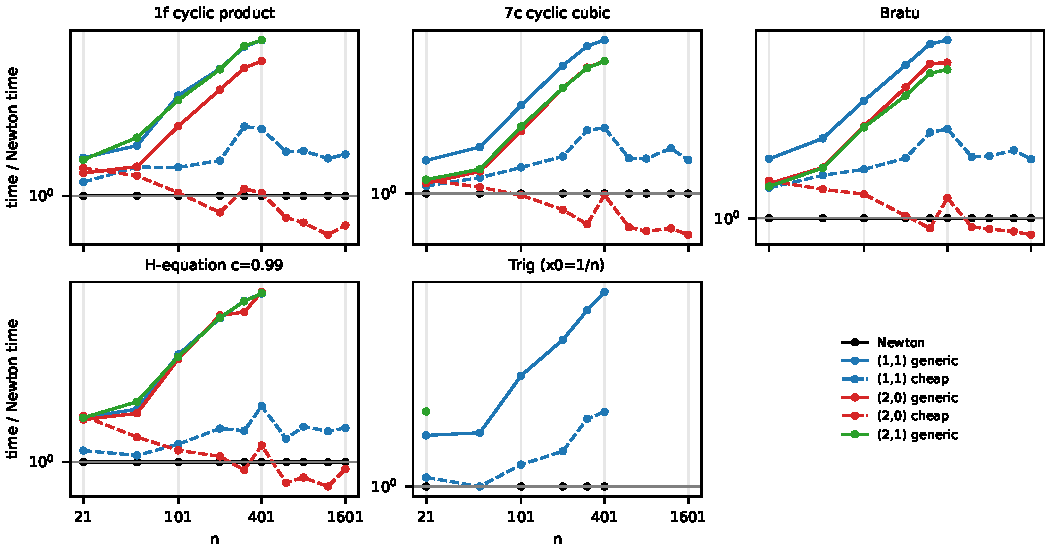
\includegraphics[width=\columnwidth]{../figures/fig_eff_rel_time.pdf}
  \Description{Six panels, one per test system, showing median wall-clock time relative to Newton against problem size n, for the generic and cheap implementations of several (p,q) members.}
  \caption{Median wall-clock time relative to Newton at the same $n$. Solid lines: generic form
  (explicit $\Lambda$). Dashed: cheap form, available for $(1,0)$, $(2,0)$, $(1,1)$. Newton is
  the horizontal reference at 1.0.}
  \label{fig:eff-rel}
\end{figure}

The generic form is never worth it in our tests: at $n=401$ it costs 3.5--5.4$\times$ Newton's
time while saving at most 1--2 iterations out of 5--8. This is exactly what the cost model
predicts --- one extra $O(n^3)$ solve per iteration is a large fixed overhead that a 25--40\%
reduction in iteration count cannot repay in double precision. The paper's own efficiency-index
comparison (its Figure 1) measures a different quantity, an abstract operations count normalized
by $\log(\text{order})/\log(\text{ops})$, which does not translate into a wall-clock statement;
our result is not a contradiction of that figure, but it is a caution against reading it as one.

The cheap forms change the picture only partially. $(1,1)$ cheap (Jarratt, two LU
factorizations, no $n$-right-hand-side solve) is consistently 1.0--2.3$\times$ Newton and never
crosses below it in any system we tried, up to $n=1601$ (Table~\ref{tab:eff-large}). $(1,0)$
cheap tracks close to Newton, between 0.8 and 1.4$\times$ depending on system and $n$, with no
consistent trend. $(2,0)$ cheap is the one case where the higher order actually wins: it drops
below Newton's time for $n\gtrsim600$ on four of the five systems, reaching 0.68--0.95$\times$
Newton's time at $n=1601$ (Table~\ref{tab:eff-large}), because it needs one fewer iteration than
$(1,0)$ for the same per-iteration cost once $n$ is large enough that the $O(n^3)$ factorization
dominates over the smaller per-iteration overhead of the extra matrix-vector product. This is a
genuine, reproducible speed-up, but it is narrow: it needs $q=0$ (so $B_{p,q}$ is never formed),
the cheap vector-recursion form (not the form a direct reading of the paper would produce), and
$n$ in the hundreds before it shows up.

\begin{table}[t]
\caption{Cheap forms at large $n$ (801 and 1601 shown; 601 and 1201 follow the same trend):
iterations / median time (ms); figure in parentheses is time relative to Newton at the same
$n$.}
\label{tab:eff-large}
\footnotesize
\setlength{\tabcolsep}{4pt}
\begin{tabular}{llcccc}
\toprule
system & n & Newton & (1,0) cheap & (2,0) cheap & (1,1) cheap \\
\midrule
1f cyclic product & 801 & 6 / 77 & 5 / 73 (0.94) & 4 / 59 (0.77) & 4 / 120 (1.56) \\
1f cyclic product & 1601 & 6 / 448 & 5 / 410 (0.92) & 4 / 334 (0.75) & 4 / 674 (1.50) \\
7c cyclic cubic & 801 & 8 / 91 & 6 / 74 (0.82) & 5 / 64 (0.70) & 5 / 127 (1.39) \\
7c cyclic cubic & 1601 & 8 / 602 & 6 / 495 (0.82) & 5 / 407 (0.68) & 5 / 829 (1.38) \\
Bratu & 801 & 5 / 59 & 4 / 51 (0.88) & 4 / 53 (0.90) & 4 / 106 (1.81) \\
Bratu & 1601 & 5 / 379 & 4 / 326 (0.86) & 4 / 324 (0.85) & 4 / 664 (1.75) \\
H-equation c=0.99 & 801 & 7 / 92 & 5 / 81 (0.88) & 5 / 82 (0.89) & 4 / 119 (1.30) \\
H-equation c=0.99 & 1601 & 7 / 565 & 5 / 516 (0.91) & 5 / 536 (0.95) & 4 / 726 (1.29) \\
\bottomrule
\end{tabular}

\end{table}

On the trigonometric system, only Newton and $(1,1)$ converge at every size we tried; $(1,0)$,
$(0,1)$ and $(2,1)$ hit the 60-iteration cap without converging, and $(2,0)$ diverges within one
or two steps. This is specific to that system's Jacobian structure near the chosen start point,
not a general property of higher-$(p,q)$ members --- the same members converge normally on the
other four systems --- but it is a reminder that a higher nominal order is not a robustness
guarantee.

\subsection{Robustness under ill-conditioning}

\begin{figure}[t]
  \centering
  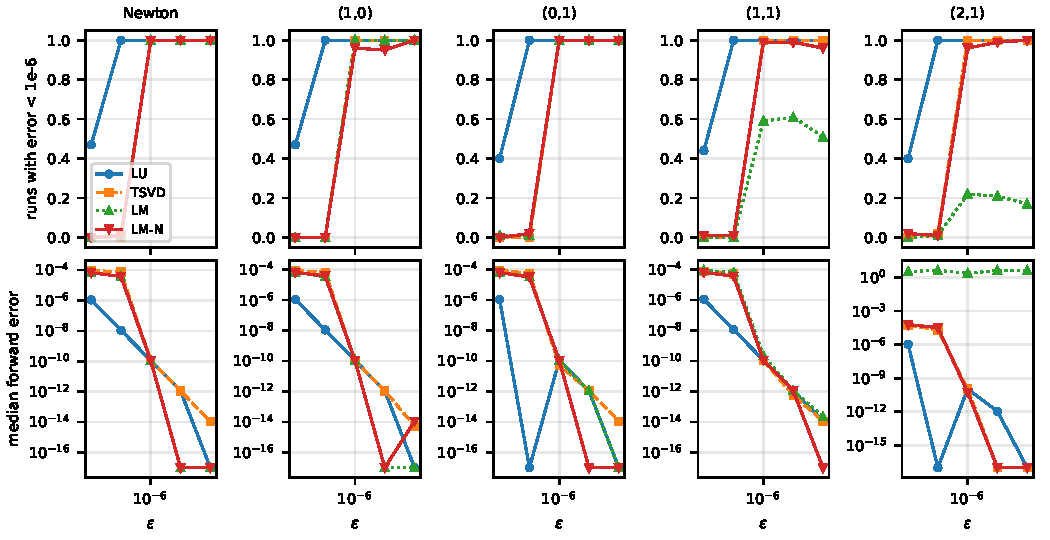
\includegraphics[width=\columnwidth]{../figures/fig_rob_nearsing.pdf}
  \Description{Five panels, one per method, showing success rate and median forward error against epsilon for LU, TSVD, LM and LM-N solves on the near-singular test system.}
  \caption{Near-singular system, $\det F'(\mathrm{root})=\epsilon$. Top: fraction of 100 random
  starts landing within $10^{-6}$ of the root. Bottom: median forward error. TSVD threshold is
  fixed at $10^{-8}$ relative.}
  \label{fig:rob-nearsing}
\end{figure}

Figure~\ref{fig:rob-nearsing} shows the near-singular sweep. Three findings, all visible directly
in the plot:

\begin{itemize}
\item \textbf{LU is fine down to about $\epsilon=10^{-6}$, then degrades.} At $\epsilon=10^{-8}$
  LU still reaches 100\% success for every $(p,q)$; at $\epsilon=10^{-10}$ it drops to 40--47\%
  and its median forward error grows to $10^{-5}$--$10^{-6}$. This is ordinary conditioning
  behaviour, not a defect of the higher-order members specifically.
\item \textbf{LM fails well before LU does, for every $(p,q)$, including plain Newton.} At
  $\epsilon\le10^{-8}$, LM's success rate is 0--1\% even for Newton itself. The damped solve
  $(J^\top J+\lambda I)^{-1}J^\top f$ with $\lambda=\|f\|^2$ becomes nearly singular in exactly
  the same direction as $J$ once $\epsilon$ is that small, so damping does not rescue it. Our
  original hypothesis, that only the $q\ge1$ members' \emph{extra} solve for $\Lambda$ breaks
  under LM, is only part of the story: at moderate $\epsilon$ ($10^{-2}$ to $10^{-6}$) that
  hypothesis holds --- LM-N (exact solve for $\Lambda$, damped solve for the Newton direction
  only) lifts $(2,1)$'s success rate from 17--22\% to 96--100\% --- but at $\epsilon\le10^{-8}$
  LM-N fails too, because by then the Newton-direction solve itself, not the $\Lambda$ solve, is
  the failure point, and that affects every $(p,q)$ including Newton.
\item \textbf{TSVD is exactly as good as LU is where LU works, and no better where LU has
  already failed}, because with a fixed relative threshold of $10^{-8}$, TSVD keeps the smallest
  singular value once $\epsilon>10^{-8}$ and discards it once $\epsilon<10^{-8}$, at which point
  it throws away the direction needed to reach the true root and converges to the wrong point
  (Figure~\ref{fig:tsvd-thresh}: at $\epsilon=10^{-10}$ or $10^{-8}$, raising the threshold to
  $10^{-10}$ or below restores 100\% accuracy). TSVD is not intrinsically more robust than LU
  here; it only helps once its threshold is set below $\epsilon$, which requires knowing
  $\epsilon$ in advance.
\end{itemize}

\begin{figure}[t]
  \centering
  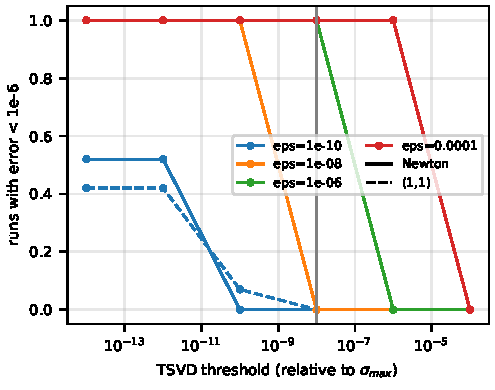
\includegraphics[width=\columnwidth]{../figures/fig_tsvd_threshold.pdf}
  \Description{Line plot of TSVD success rate against the relative singular-value threshold, for four fixed values of epsilon, showing the threshold must be set below epsilon to succeed.}
  \caption{TSVD success rate as a function of the relative singular-value threshold, for four
  fixed $\epsilon$. The vertical line marks the threshold ($10^{-8}$) used elsewhere in this
  report.}
  \label{fig:tsvd-thresh}
\end{figure}

\begin{table*}[t]
\caption{Exactly-singular systems: accurate\% (converged\%) / median iterations, 100 random
starts per row.}
\label{tab:natural}
\small
\begin{tabular}{llccccc}
\toprule
system & solver & Newton & (1,0) & (0,1) & (1,1) & (2,1) \\
\midrule
CosDiag & LU & 100 (100) / 28 & 100 (100) / 21 & 100 (100) / 19 & 100 (100) / 18 & 100 (100) / 15 \\
CosDiag & TSVD & 100 (100) / 28 & 100 (100) / 21 & 100 (100) / 19 & 100 (100) / 18 & 100 (100) / 15 \\
CosDiag & LM & 100 (100) / 32 & 100 (100) / 23 & 100 (100) / 20 & 0 (0) / 200 & 0 (0) / 200 \\
CosDiag & LM-N & 100 (100) / 32 & 100 (100) / 25 & 100 (100) / 23 & 100 (100) / 22 & 100 (100) / 20 \\
Powell & LU & 100 (100) / 42 & 100 (100) / 30 & 100 (100) / 27 & 100 (100) / 22 & 100 (100) / 20 \\
Powell & TSVD & 100 (100) / 98 & 100 (100) / 80 & 100 (100) / 76 & 100 (100) / 15 & 100 (100) / 14 \\
Powell & LM & 100 (0) / 36 & 99 (0) / 26 & 100 (6) / 22 & 0 (0) / 200 & 0 (0) / 200 \\
Powell & LM-N & 100 (0) / 36 & 95 (0) / 28 & 99 (0) / 26 & 100 (0) / 22 & 100 (0) / 21 \\
H-eq c=1 & LU & 0 (0) / 200 & 0 (0) / 200 & 2 (2) / 200 & 0 (0) / 200 & 1 (1) / 200 \\
H-eq c=1 & TSVD & 100 (100) / 26 & 100 (100) / 19 & 100 (100) / 17 & 100 (100) / 14 & 100 (100) / 13 \\
H-eq c=1 & LM & 7 (7) / 50 & 3 (3) / 40 & 1 (1) / 30 & 0 (0) / 200 & 0 (0) / 200 \\
H-eq c=1 & LM-N & 7 (7) / 50 & 1 (1) / 44 & 1 (1) / 43 & 4 (4) / 39 & 2 (2) / 37 \\
\bottomrule
\end{tabular}

\end{table*}

Table~\ref{tab:natural} gives success rates (accurate / converged, both as \%) and median
iterations on the three exactly-singular systems. Here the picture is sharper and, for the
H-equation at $c=1$, striking: \textbf{LU never succeeds} (0--2\% across every $(p,q)$, and it
does not fail cleanly --- it runs to the 200-iteration cap without meeting the stopping rule).
\textbf{TSVD succeeds every single time} for every $(p,q)$, because the Jacobian's null space is
one-dimensional and constant in direction near the root, so a fixed relative threshold reliably
separates it from the rest of the spectrum. On Powell's function and the cosine-diagonal system,
LU is unexpectedly fine (100\% both measures for every $(p,q)$); TSVD matches it but needs many
more iterations at low order (76--98 vs.\ 27--42) since the pseudo-inverse changes the local
convergence rate away from the root. LM and LM-N are unreliable on all three systems in the same
way as in the near-singular sweep: high forward-error accuracy sometimes, near-zero rate of
actually satisfying the stopping criterion, because the damping keeps perturbing the step near
the solution rather than letting it settle.

\textbf{Overall solver recommendation from these experiments:} LU is a reasonable default and is
cheaper than TSVD when the Jacobian is not exactly singular. Switch to TSVD specifically when the
Jacobian has a known, low-dimensional null space (a genuinely singular problem), and set its
threshold below the smallest genuine singular value you expect, not at a generic default. LM, at
least in the plain $\lambda=\|f\|^2$ form we tested, is not a safe default for this family of
methods; it degrades before LU does rather than after.

\section{Conclusion and Future Work}

The base paper's convergence-order claims held up in every reproduction we ran, with one
unresolved discrepancy of one iteration in three of fifteen validation cases (Section 4.1) and
one case of order exceeding the proven bound rather than falling short of it (Section 4.2),
neither of which affects the paper's central theorem. The two questions the paper leaves open
have concrete answers in our tests: a literal, direct implementation of a higher-$(p,q)$ member
is never faster than Newton in wall-clock time in double precision, for any system or size we
tried, because forming $\Lambda$ costs an extra $O(n^3)$ solve that a modest reduction in
iteration count cannot repay; an algebraically equivalent implementation that avoids forming
$\Lambda$ removes most of that overhead, and for $(2,0)$ specifically becomes genuinely faster
than Newton once $n$ is in the hundreds. On robustness, plain LU is adequate for moderately
ill-conditioned Jacobians and fails completely on exactly singular ones; TSVD fixes that but only
if its threshold is set correctly for the problem; and Levenberg--Marquardt damping, in the form
we tested, is not a reliable default for this family at all, failing before LU does rather than
extending its range.

Limitations: our efficiency comparison used only LU-based solves and only five systems, all with
either a dense or a fixed sparsity pattern; a sparse-Jacobian benchmark could change the cost
model materially since the $O(n^3)$ term that dominates our conclusion is specific to dense
factorization. The cheap form is only available for $q=0$ and for $(1,1)$; whether a similarly
cheap recursion exists for other $q\ge1$ members is an open algebraic question we did not
pursue. The LM variant we used is the simplest textbook choice
of damping parameter~\cite{levenberg1944,marquardt1963}; an adaptive schedule for $\lambda$
might change the robustness comparison and is worth testing before concluding LM is unusable
here. Finally, the one-iteration mismatch in Section 4.1 is unresolved; matching the original
authors' code, if it becomes available, would settle whether it is a stopping-rule detail or
something else.

\section*{Code and Reproducibility}
Source code, test suite, and every CSV result underlying this report:
\url{https://github.com/sleepy-panda-ndroid/Pade-Newton-Numerical-Project-4-1}.
Reproduce with \texttt{python run\_all.py} (full run,
15--25 minutes single-threaded) or \texttt{python run\_all.py~-\/-quick} (smoke test, 1--2
minutes); see \texttt{README.md}.

\bibliographystyle{ACM-Reference-Format}
\bibliography{references}

\end{document}
